%************************************************
\chapter{Introduction}\label{ch:introduction}
%************************************************
\section{Motivation}
In recent years, there has been a rise in the use of neuroimaging in the clinical practice. It has improved and speeded the procedure of diagnostic, providing unprecedented insight into the brain. Neuroimaging is very extended in research as well. Different fields such as psychiatry, neurology, psychology, behavioural science or biology make extensive use of brain imaging in their studies. 

The basis of most of these studies is common: a procedure by which a representative set of subjects is recruited, the fulfilment of an experiment on (or by) each subject and a statistical analysis of the acquired data. Particularly, when studying a certain disease, it is common to recruit subjects affected by the disease and a matched population of non-affected, healthy subjects, usually known as \acp{CTL}. Then, in this typical example, both affected and \acp{CTL} are scanned, and brain anatomy or function is analysed using statistical tools. The result of this analysis is frequently a list of significant differences between structure or function that could be linked to the disease. 

\acf{CAD} systems provide a set of tools to help setting up and performing these studies. It is currently a thriving area of research involving multidisciplinary teams, combining computer science, mathematics, medicine, artificial intelligence, statistics, machine learning, and many others \cite{Martinez-Murcia2016}. The main aim is to assist clinicians in the procedure of diagnosis and study of the diseases by providing software that can effectively recognize disease patterns, characterize differences and make predictions. 

One fundamental issue often found in this studies is the sample size. The number of subjects frequently ranges from tens to hundreds, whereas the number of features (namely voxels) to be analysed can add up to millions. This causes the so-called \emph{Small Sample Size Problem} \cite{Duin2000} which negatively affects the statistical power of any experiment performed using these datasets \cite{Button2013}. 

\begin{figure}
\centering
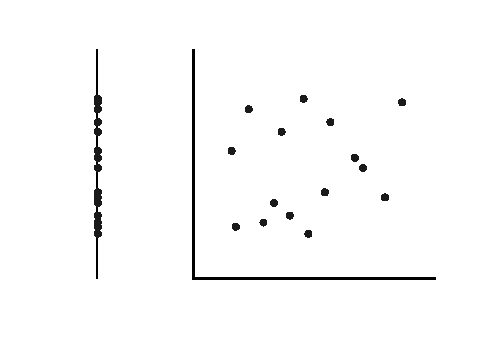
\includegraphics[width=0.6\linewidth]{Graphics/ch1/smallsample}
\caption[Illustration of one and two-dimensional spaces.]{Illustration of the separation between points in one-dimensional and two-dimensional spaces.}
\label{fig:smallsample}
\end{figure}


\section{The Small Sample Size Problem}\label{sec:smallsamplesize}
The \textit{Small Sample Size Problem} refers to a problem that arises when the ratio between the number of subjects and the number of features is large. Think of, \eg, 15 points in a one-dimensional line, as in Figure~\ref{fig:smallsample}. If we think of a subject as a vector, we would have 15 subjects in a one-dimensional space. Now, imagine that we add a second dimension. It is easy to see that our subjects would be more distant than in the one-dimensional line. And the same would happen if we move to three, ten or thousands of dimensions. The farther our points are, the more difficult is for a statistical tool to extract information. That is what we call \textit{almost empty spaces} \cite{Duin2000,Stoeckel04}, in contrast to \textit{dense spaces}, where points are closer. 

Neuroimaging provides hundreds of thousands, or even millions of voxels, in what could mean millions of features. That implies that any calculation performed in those almost empty spaces will eventually lack information. This implies a loss of statistical power of the methods used, usually producing false negatives (the system is unable to detect real signal) and false positives (the system detects signal where there is not). These are known in statistics as Type I and Type II errors respectively. 

In differential diagnosis studies, the small sample size problem leads to wrong conclusions about where real differences are located. This, in addition to untracked confounding variables are some of the fundamental sources of non-re\-pro\-du\-ci\-bi\-li\-ty un current neuroimaging studies \cite{Button2013}. 

The solution might seem straightforward: increase sample size. But this is not always possible, since neuroimaging studies do their best at recruiting as many people as they can with a limited budget. Many efforts have been put into establishing multi-centre collaborations that allow the recruitment of a larger population, but despite offering a higher statistical power, these studies still suffer from a number of confounding variables such as population bias or scanner differences \cite{haar2014anatomical}. In chapters~\ref{ch:swpca} and \ref{ch:simulation} we explore different approaches to this solution. 

Another option involves reducing the number of features, via feature selection or feature extraction. This has been widely used in computed-aided methodology for neuroimaging very successfully \cite{DeMartino2007,Xu2009,Gorriz2010,Illan2011,Martinez-Murcia2016}, and solutions using this approach will be presented in chapters~\ref{ch:decomposition}, \ref{ch:texture} and \ref{ch:sbm}. 

The Small Sample Size problem is directly related to the \textit{Curse of Dimensionality} \cite{Krishnaiah1982}, which proves that, in contrast to what might be expected, once a certain classifier performance has been achieved, it holds or even decreases when feeding more features to the classifier. The problem also affects statistical hypothesis testing, a tool widely used for inference in neuroimaging, in what is known as the \textit{Multiple Comparisons} problem \cite{Benjamini2010}, a particular field that is still being studied. 

\section{Aims and Objectives}\label{sec:overview}
This thesis aims to contribute new approaches to overcome the small sample size problem in neuroimaging. This can lead to more accurate \ac{CAD} systems by reducing the number of false positives, increasing the reliability of their results. 

We will take two different approaches, as commented in the previous section: increasing the sample size and reducing the feature space. Therefore, we can define the following objectives: 

\begin{itemize}
	\item Develop and evaluate algorithms that reduce the feature space, in which is usually known in the field as feature extraction and feature selection strategies. 
	\item Develop and evaluate new strategies to increase the sample size in neuroimaging studies. 
\end{itemize}

Most of the studies in the literature focus on the first objective. Feature extraction algorithms that use \acf{PCA} \cite{Khedher2015,Towey2011} or \acf{PLS} \cite{Segovia2013}, among others, are widely studied. We have developed three different approaches to those:

\begin{itemize}
	\item A combination of image decomposition algorithms and feature selection. In this approach we used three statistical tests to select the most significant voxels from the images, and then applied \acf{FA} and \acf{ICA} to decompose the data and significantly reduce their feature space. 
	\item A feature extraction based on texture analysis. 
	\item A novel strategy called \acf{SBM}. This feature extraction technique uses a spherical coordinate system to map statistical measures to a bidimensional plane. It builds paths used as feature selection vectors where several measures are computed. 
\end{itemize}

On the other hand, we have evaluate newer ways to safely increase sample size in neuroimaging studies. We have developed: 
 \begin{itemize}
 	\item A system to reduce undesired variance in structural multicentre studies, called \acf{SWPCA}. This system is intended to reduce the amount of false positives in large collaborations, providing more homogeneous images and improving their statistical power. 
 	\item An algorithm to simulate functional brain images using existing data, and therefore, increase sample size. 
 \end{itemize}

\begin{figure}
	\centering
	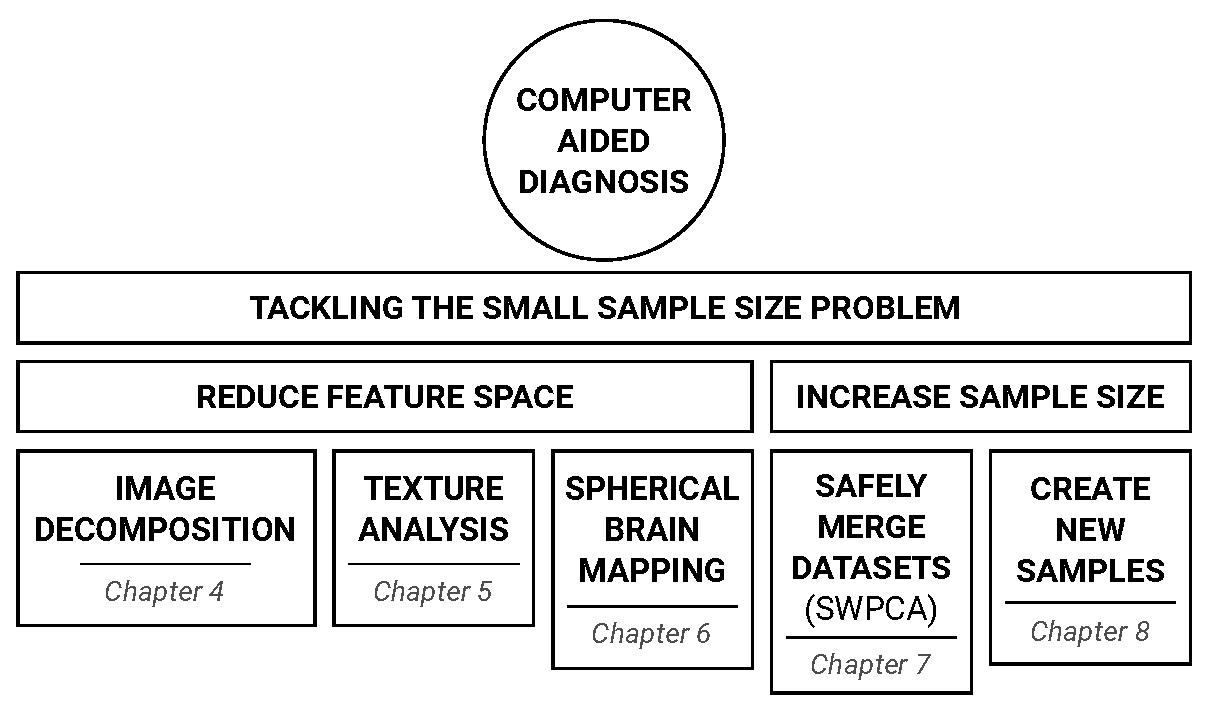
\includegraphics[width=0.7\linewidth]{Graphics/ch1/outline}
	\caption[Structure of the thesis.]{Structure and connexions between the different strategies proposed in this thesis, organized by chapters and parts.}
	\label{fig:outline}
\end{figure}


\section{Organization of this Thesis}
This thesis work is organized in four parts plus appendices, each of which is subdivided in several chapters. In the first part, we introduce the motivations and main aims of this work (chapter~\ref{ch:introduction}), examine the state of the art in medicine, neuroimaging and \ac{CAD} systems (chapter~\ref{ch:stateofart}) and present a general methodology that will be followed throughout this thesis, including preprocessing and evaluation (chapter~\ref{ch:preprocessing}). 

Parts \ref{part:feature} and \ref{part:increase} refers to each of the solutions outlined in the previous section, and disaggregated in Figure~\ref{fig:outline}. In part~\ref{part:feature} we focus on the feature reduction techniques, including decomposition methods (chapter~\ref{ch:decomposition}), texture analysis (chapter~\ref{ch:texture}), and the novel algorithm Spherical Brain Mapping (chapter~\ref{ch:sbm}). On the other hand, Part~\ref{part:increase} is focused on two different strategies used to increase the sample size: the Significance Weighted Principal Component Analysis algorithm (chapter~\ref{ch:swpca}), used to safely merge structural images acquired at different centres, and a neuroimage simulation algorithm (chapter~\ref{ch:simulation}) that can be used to extend existing functional datasets. 

Finally, in Part~\ref{part:dicussion} we provide a general discussion of the results presented in this thesis, conclusions about the methods and prospective work that could be performed with this basis. 

\section{Contributions}
Some ideas and figures have appeared previously in the following publications, that we divide here in articles, conference presentations and book chapters. 

%\noindent Put your publications from the thesis here. The packages \texttt{multibib} or \texttt{bibtopic} etc. can be used to handle multiple different bibliographies in your document.

\begin{refsection}[ownpubs]
	\small
	\nocite{*} % is local to to the enclosing refsection
	\newrefcontext[sorting=ydnt]
	\subsection{Articles}
	\printbibliography[env=nolabelbib,heading=none,keyword=own, title={Articles}, type=article]
	\subsection{Conferences}
	\printbibliography[env=nolabelbib,heading=none,keyword=own, title={Conferences}, type=inproceedings]
	\subsection{Books}
	\printbibliography[env=nolabelbib,heading=none,keyword=own, title={Books}, type=inbook]
\end{refsection}


% DONE